\documentclass[14pt]{beamer}
\usetheme{Montpellier}
\usecolortheme{beaver}

\usepackage{amsmath, amssymb, ../../vimacros, hyperref, enumerate}
\usepackage{../../pdfpcnotes}
\usepackage[round]{natbib}

\usepackage{multicol}
\usepackage{physics}
\usepackage{xfrac}

\hypersetup{breaklinks=true, colorlinks=true, linkcolor=blue, citecolor=blue, urlcolor=blue}

\usepackage{tikz}
\usetikzlibrary{bayesnet}

\beamertemplatenavigationsymbolsempty

\title{Welcome and Introduction}
\date{}
\author[Schulz and Aziz]{Philip Schulz and Wilker Aziz \\
\url{https://github.com/philschulz/VITutorial}}

\setbeamertemplate{footline}[frame number]

\begin{document}

\frame{\titlepage}

\begin{frame}{About us \ldots}
\begin{block}{Wilker Aziz}
\begin{itemize}
\item Assistant Professor at UvA-ILLC
\item VI, sampling methods, NLP
\end{itemize}
\end{block}

\begin{block}{Philip Schulz}
\begin{itemize}
\item Applied Scientist at Amazon
\item VI, machine translation, Bayesian models
\end{itemize}
\end{block}
\end{frame}

\begin{frame}{Why are we here today?}

Because NN models work \\ \pause
~ but they may struggle with
\begin{itemize}
	\item lack of supervision
	\item partial supervision
	\item lack of inductive bias
\end{itemize}
\pause

In such cases, we usually turn to probabilistic models \\ \pause
~ but it turns out NNs and PGMs do not go along
\begin{itemize}
	\item well... \pause that's no longer true!
\end{itemize}

\end{frame}

\begin{frame}{What are you getting out of this today?}

As we progress we will
\begin{itemize}
	\item develop a shared vocabulary to talk about generative models powered by NNs
	\item derive crucial results step by step
\end{itemize}

\pause

Goal
\begin{itemize}
	\item you should be able to navigate through fresh literature
	\item and start combining probabilistic models and NNs
\end{itemize}

\end{frame}




\begin{frame}{Supervised problems}

We have data $x^{(1)}, \ldots,  x^{(N)}$ \textcolor{gray}{~ e.g. sentences, images} \\
generated by some {\bf unknown} procedure 
which we assume can be captured by a probabilistic model


\begin{itemize}
	\item with {\bf known} probability (mass/density) function e.g.
	\begin{align*}
    X \sim \Cat(\alert{\theta_1}, \alert{\ldots}, \alert{\theta_K}) & & \text{or} & & X \sim \mathcal N(\alert{\theta_\mu}, \alert{\theta^2_\sigma})
    \end{align*}    
\end{itemize}
\pause
and \alert{estimate parameters $\theta$}  that assign maximum likelihood $p(x^{(1)}, \ldots, x^{(N)}|\theta)$ to observations

\end{frame}


\begin{frame}{Supervised NN models}

Let $y$ be all side information available\\
~ e.g. deterministic \emph{inputs/features/predictors}

~

Have neural networks predict parameters of our probabilistic model
	\begin{align*}
    X|y \sim \Cat(\pi_{\alert \theta}(y)) & & \text{or} & & X|y \sim \mathcal N(\mu_{\alert \theta}(y), \sigma_{\alert \theta}(y)^2)
    \end{align*}
~ and proceed to \alert{estimate parameters $\theta$}  of the NNs %via MLE % that assign maximum likelihood to observations



\end{frame}



\begin{frame}{Graphical model}

\begin{columns}
\begin{column}{0.6\textwidth}

Random variables
\begin{itemize}
	\item observed data \\
	$x^{(1)}, \ldots, x^{(N)}$
\end{itemize}

Deterministic variables
\begin{itemize}
	\item inputs or predictors \\
	$y^{(1)}, \ldots, y^{(N)}$
	\item model parameters $\theta$
\end{itemize}

\end{column}
\begin{column}{0.2\textwidth}
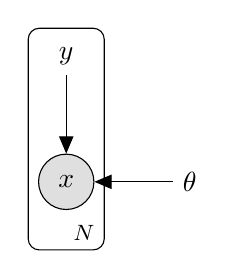
\begin{tikzpicture}
\node[obs] (x) {$ x $};
\node[above=of x] (y) {$ y $};
\node[right=of x] (theta) {$ \theta $};
\edge{y,theta}{x};

\plate {data} {(y) (x)} {$ N $};
\end{tikzpicture}
\end{column}

\end{columns}


\end{frame}


\begin{frame}{Multiple problems, same language}



\begin{small}

\begin{columns}
\begin{column}{0.3\textwidth}
\scalebox{0.8}{
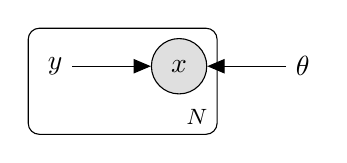
\begin{tikzpicture}
\node[obs] (x) {$ x $};
\node[left=of x] (y) {$ y $};
\node[right=of x](theta) {$\theta$};
\edge{theta,y}{x};

\plate {data} {(y)(x)} {$ N $};
\end{tikzpicture}
}
\end{column}
\begin{column}{0.6\textwidth}
\alert{(Conditional) Density estimation}
\end{column}

\end{columns}

\begin{tabular}{p{2cm} p{4cm} p{4cm}}
 & Side information ($y$) & Observation ($x$) \\
Parsing &   \textcolor{gray}{a sentence} & \textcolor{black}{its syntactic/semantic parse tree/graph} \\
&&\\
Translation &  \textcolor{gray}{a sentence} & \textcolor{black}{its translation} \\
&&\\
Captioning &  \textcolor{gray}{an image} & \textcolor{black}{caption in English} \\
&&\\
Entailment  & \textcolor{gray}{a text and hypothesis} & \textcolor{black}{entailment relation}
\end{tabular}
\end{small}

\end{frame}


\begin{frame}{Task-driven feature extraction}

Often our side information is itself some high dimensional data
\begin{itemize}
	\item $y$ is a sentence and $x$ a tree
	\item $y$ is the source sentence and $x$ is the target
	\item $y$ is an image and $x$ is a caption
\end{itemize}
and part of the job of the NNs that parametrise our models is to also \alert{deterministically} encode that input in a low-dimensional space

%~
%\begin{itemize}
%	\item NNs parameterise probability functions
%	\item NNs predict parameters of a probabilistic model
%\end{itemize}

\end{frame}


\begin{frame}{NN as efficient parametrisation}

From a statistical point of view, NNs do not generate data\\
\begin{itemize}
	\item \alert{they parametrise distributions} that \\
	\emph{by assumption} govern data
	\item compact and efficient way to \alert{map from complex side information to parameter space}
\end{itemize}

\vspace{10pt}

\pause
Prediction is done by a decision rule outside the statistical model
\begin{itemize}
	\item e.g. argmax, beam search
\end{itemize}

\end{frame}



\begin{frame}{Maximum likelihood estimation}

Let $p(x|\theta)$ be the probability of an observation $x$\\
~and $\theta$ refer to all of its parameters \\
%~e.g. parameters of NNs involved

~ \pause

Given a dataset $x^{(1)}, \ldots, x^{(N)}$ of i.i.d. observations, \pause
the log-likelihood function gives us a criterion for parameter estimation
\begin{equation*}
\begin{aligned}
\mathcal L(\theta|x^{(1:N)}) &= \pause \log \prod_{s=1}^N p(x^{(s)}|\theta) 
 = \pause \sum_{s=1}^N \log p(x^{(s)}|\theta)
\end{aligned}
\end{equation*} 


\end{frame}

\begin{frame}{MLE via gradient-based optimisation}

If the log-likelihood is {\bf differentiable} and  {\bf tractable}\\
~then backpropagation gives us the gradient
\begin{small}
\begin{equation*}
\begin{aligned}
\grad_\theta \mathcal L(\theta|x^{(1:N)}) &= \pause \grad_\theta \sum_{s=1}^N \log p(x^{(s)}|\theta) 
 &= \pause \sum_{s=1}^N \grad_\theta \log p(x^{(s)}|\theta)
\end{aligned}
\end{equation*}
\end{small}  \pause

and we can update $\theta$ in the direction
\begin{equation*}
\gamma \grad_\theta \mathcal L(\theta|x^{(1:N)})
\end{equation*}
to attain a local maximum of the likelihood function

\end{frame}


\begin{frame}{Big Data}
\pnote{Q: Why computing the exact gradient is inconvenient?} 

For large \alert{$N$}, computing the gradient is inconvenient
\begin{small}
\begin{equation*}
\begin{aligned}
\grad_\theta \mathcal L(\theta|x^{(1:N)}) &=   \underbrace{\sum_{s=1}^{\alert{N}} \grad_\theta \log p(x^{(s)}|\theta)}_{\text{too many terms}} \\ \pause
&=   \sum_{s=1}^{\alert{N}} \textcolor{blue}{\frac{1}{ N} } N \grad_\theta \log p(x^{(s)}|\theta) \\ \pause
&= \sum_{s=1}^{\alert{N}}\textcolor{blue}{\mathcal U(s|\sfrac{1}{N})}  N \grad_\theta \log p(x^{(s)}|\theta) \\ \pause
&= \mathbb E_{S\sim \mathcal U(\sfrac{1}{N})}\left[ N \grad_\theta  \log p(x^{(S)}|\theta)\right]
\end{aligned}
\end{equation*} 
\end{small}

$S$ selects data points uniformly at random



\end{frame}

\begin{frame}{Stochastic optimisation}

\pnote{Q: Why should we like expected gradients?} 

For large $\alert{N}$, we can use a gradient estimate 
\begin{small}
\begin{equation*}
\begin{aligned}
\grad_\theta \mathcal L(\theta|x^{(1:N)}) 
 &=  \underbrace{\mathbb E_{S\sim \mathcal U(\sfrac{1}{N})}\left[ N \grad_\theta  \log p(x^{(S)}|\theta)\right]}_{\text{expected gradient :)}} \\ \pause
 &\overset{\text{MC}}{\approx} \frac{1}{M} \sum_{m=1}^M N  \grad_\theta \log p(x^{(s_m)}|\theta) \\
 &S_m \sim \mathcal U(\sfrac{1}{N})
\end{aligned}
\end{equation*}
\end{small}  \pause
and take a step in the direction
\begin{small}
\begin{equation*}
\gamma \frac{N}{M} \underbrace{\grad_\theta \mathcal L(\theta|x^{(s_1:s_M)})}_{\text{\alert{stochastic gradient}}}
\end{equation*}
\end{small}
where $x^{(s_1:s_M)}$ is a random mini-batch of size $M$


\end{frame}




\begin{frame}{DL in NLP recipe}


%Vast majority of papers published at ACL

%\begin{small}
%\begin{figure}
%\scalebox{0.8}{
%\begin{tikzpicture}
%\node[obs] (x) {$ x $};
%\node[left=of x] (phi) {$ \phi $};
%\factor[left=of x] {f} {below:$f_w$} {phi} {x} ; 
%%\edge{phi}{x} ;
%\plate {data} {(x)(phi)} {$ N $};
%\end{tikzpicture}
%}
%\end{figure}
%\end{small}
	Maximum likelihood estimation
	\begin{itemize}
		\item  tells you which \alert{loss} to optimise \\
		(i.e. negative log-likelihood)
	\end{itemize}
	
	Automatic differentiation (\emph{backprop})
	\begin{itemize}
		\item ``give me a tractable forward pass and I will give you \alert{gradients}''
	\end{itemize}
	
	Stochastic optimisation powered by backprop
	\begin{itemize}
		\item general purpose gradient-based optimisers
	\end{itemize}

\end{frame}


\begin{frame}{Constraints}

	Differentiability
	\begin{itemize}
		\item intermediate representations must be continuous
		\item activations must be differentiable
	\end{itemize}

	Tractability
	\begin{itemize}
		\item the likelihood function must be evaluated exactly, thus it's required to be tractable
	\end{itemize}


%, any intractable likelihood will leave us in bad territory because
%\begin{itemize}
%	\item stochastic optimisation requires gradient estimates
%	\item which must be unbiased (forget greedy techniques)
%	\item and some estimation techniques are not differentiable (forget MC sampling)
%\end{itemize}

\end{frame}




\begin{frame}{When do we have intractable likelihood?}

{\bf Unsupervised problems} contain unobserved random variables\\ 
\begin{equation*}
p(x, z|\theta) = \overbrace{p(z)}^{\text{prior}} \underbrace{p(x|z, \theta)}_{\text{observation model}}
\end{equation*}

~ \pause

thus assessing the marginal likelihood requires \alert{marginalisation of latent variables} 
\begin{equation*}
p(x|\theta) = \int p(x, z|\theta) \dd{z} = \int p(z)p(x|z, \theta) \dd{z} 
\end{equation*}

\end{frame}





\begin{frame}{Latent variable model}

%Unsupervised problems contain latent random variables\\ 
\begin{columns}
\begin{column}{0.6\textwidth}
Latent random variables
\begin{itemize}
	\item unobserved 
	\item or unobservable
\end{itemize}
\end{column}
\begin{column}{0.2\textwidth}
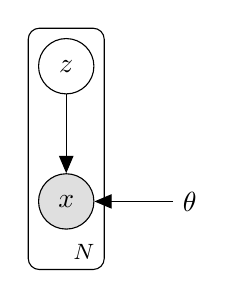
\begin{tikzpicture}
\node[obs] (x) {$ x $};
\node[latent,above=of x] (z) {$ z $};
\node[right=of x] (theta) {$ \theta $};
\edge{z,theta}{x};

\plate {data} {(z)(x)} {$ N $};
\end{tikzpicture}

\end{column}
\end{columns}

~ \pause


A joint distribution over data and unknowns
\begin{equation*}
p(x, z|\theta) = p(z) p(x|z, \theta)
\end{equation*}

\end{frame}


\begin{frame}{Examples of latent variable models}

\pnote{Q: Can you think of a practical example of discrete latent and continuous observation?} 

\pnote{Q: Can you think of a practical example of continuous latent and discrete observation?} 

Discrete latent variable, continuous observation
	\begin{small}
	\begin{equation*}
	p(x|\theta) = \underbrace{\sum_{c=1}^K \Cat(c|\pi_1, \ldots, \pi_K) \underbrace{\mathcal N(x|\mu_\theta(c), \sigma_\theta(c)^2)}_{\text{forward pass}}}_{\text{{\bf too many forward passes}}}
	\end{equation*}
	\end{small} 

	\pause
	
Continuous latent variable, discrete observation
	\begin{small}
	\begin{equation*}
	p(x|\theta) = \underbrace{\int \mathcal N(z|0, I) \underbrace{\Cat(x|\pi_\theta(z))}_{\text{forward pass}} \mathrm{d}z }_{\text{\alert{{\bf infinitely many forward passes}}}}
	\end{equation*}
	\end{small}

\end{frame}

\begin{frame}{Intractable gradient}

\begin{small}
\begin{equation*}
\begin{aligned}
\grad_\theta \log p(x|\theta) \pause &= \grad_\theta \log \underbrace{\int p(x, z|\theta) \dd{z}}_{\text{marginal}} \\ \pause
&= \underbrace{\frac{1}{\int p(x, z|\theta) \dd{z}} \int \grad_\theta p(x,z|\theta) \dd{z}}_{\text{chain rule}} \\ \pause
&= \frac{1}{p(x|\theta)} \int \underbrace{p(x,z|\theta) \grad_\theta \log p(x,z|\theta)}_{\text{log-identity for derivatives}} \dd{z} \\ \pause
&= \int \alert{p(z|x, \theta)} \grad_\theta \log p(x,z|\theta) \dd{z} %\\ \pause
%&= \mathbb E_{\alert{p(z|x, \theta)}} \left[ \grad_\theta \log p(x,z|\theta) \right]
\end{aligned}
\end{equation*}
\end{small}



\end{frame}

\begin{frame}{Gradient estimates?}

\begin{equation*}
\begin{aligned}
&\grad_\theta \log p(x|\theta) = \int \alert{p(z|x, \theta)} \grad_\theta \log p(x,z|\theta) \dd{z} \\ \pause
&= \mathbb E_{\alert{p(z|x, \theta)}} \left[ \grad_\theta \log p(x,z|\theta) \right] \\ \pause
&\overset{\text{MC}}{\approx} \frac{1}{K} \sum_{k=1}^K \grad_\theta \log p(x, z_k|\theta) 
\quad \textcolor{gray}{\text{where }z_k \sim p(z|x, \theta)}
\end{aligned}
\end{equation*}

\pause But what are we sampling from exactly?

\begin{equation*}
\begin{aligned}
	p(z|x, \theta) = \pause \frac{p(x, z|\theta)}{\alert{p(x|\theta)}} % = \frac{p(z)p(x|z, \theta)}{\int p(z', x|\theta) \dd z'}
\end{aligned}
\end{equation*}

\end{frame}


\begin{frame}{But why latent variable modelling?}

Some reasons

\begin{itemize}
	\item better handle on statistical assumptions\\
	e.g. breaking marginal independence \pause
	\item organise a massive collection of data\\
	e.g. LDA	 \pause
	\item learn from unlabelled data\\
	e.g. semi-supervised learning \pause
	\item induce discrete representations\\
	e.g. parse trees, dependency graphs, alignments \pause
	%e.g. derivatives are not defined for discontinuous functions
	\item uncertainty quantification\\
	e.g. Bayesian NNs 
\end{itemize}

\end{frame}

\begin{frame}{Examples: Lexical alignment}

Generate a word $x_i$ in L1 from a word $y_{a_i}$ in L2
	\begin{equation*}
	\begin{aligned}
		P(x|y, \theta) %&= \sum_{a_1=1}^{\abs{y}}\cdots \sum_{a_{\abs{x}}=1}^{\abs{y}} \prod_{i=1}^{\abs{x}} P(a_i|y)P(x_i|y,a_i, a_{<i}) \\
		&\overset{\text{\alert{ind}}}{=} \prod_{i=1}^{\abs{x}} \sum_{a_i=1}^{\abs{y}}P(a_i|y)P(x_i|y_{\alert{a_i}}) 
		\end{aligned}
	\end{equation*}

a mixture model whose mixture components are labelled by words \hfill \textcolor{blue}{marginalisation $O(\abs{x}\abs{y})$}

\end{frame}

\begin{frame}{Examples: Rationale extraction}

Sentiment analysis based on a subset of the input
\begin{equation*}
	\begin{aligned}
		P(x|y, \theta) &= \sum_{f_1=0}^{1}\cdots \sum_{f_{\abs{y}}=0}^{1} P(x|f,y) \prod_{i=1}^{\abs{y}} \Bernoulli(f_i|\theta_{y_i}) \\
		\end{aligned}
	\end{equation*}
where $P(x|f,y)$ conditions on $y_i$ iff $f_i = 1$.

~

A factor model whose factors are labelled by words \\
\hfill \alert{marginalisation $O(2^{\abs{y}})$}

\end{frame}

\begin{frame}{Examples: Language modelling}

	A (deterministic) RNNLM aways produces the same conditional for a given prefix. Isn't it reasonable to expect the conditional to depend on what we are talking about?: e.g. \emph{Rio de Janeiro $\ldots$}
	\begin{itemize}
		\item history: \emph{was once the Brazilian capital}
		\item tourism: \emph{offers some of Brazil's most iconic landscapes}
		\item news: \emph{recently hosted the world cup final}
	\end{itemize}
	\vspace{-5pt}
	\begin{equation*}
		P(x|\theta) = \int \mathcal N(z|0, I) \prod_{i=1}^{\abs{x}} P(x_i|z, x_{<i}, \theta)
	\end{equation*}

\end{frame}


\begin{frame}{Deep Generative Models}

Probabilistic models parametrised by neural networks
\begin{itemize}
	\pause
	\item explicit modelling assumptions\\
	one of the reasons why there's so much interest	
	\pause
	\item but requires efficient inference\\
	\pause
	\alert{which is the reason why we are here today}
\end{itemize}

\end{frame}



\end{document}
